
%----------------------------------------------------------------------------------------
%	PROBLEM 1
%----------------------------------------------------------------------------------------

% To have just one problem per page, simply put a \clearpage after each problem

\begin{homeworkProblem}
Une approche très répandue dans l’étude de la propagation des logiciels malveillants
consiste à développer un modèle déterministe basé sur les concepts de compartiments et
de règles [2]. Les compartiments servent à diviser la population étudiée en différentes
classes et les règles à définir les conditions de transition entre chacune des classes.
\begin{homeworkSection}{1.1}
En vous basant sur l’article « Optimising Networks Against Malware » [3], quel
modèle comportemental (SI, SIS, SIR) s’appliquerait et pourquoi? Justifiez votre réponse
en expliquant quel modèle s’applique et pourquoi les autres modèles ne s’appliquent pas.

\problemAnswer{ % Answer
Le modèle comportemental qui s'applique dans le cas de l'article est le modèle SI.
En effet dans le troisième paragraphe, il est indiqué d'un seul état de transition est possible, à savoir de susceptible à infecté.
De plus au cours de l'expérience, aucune contre mesure n'est appliqué et on ne fait aucune opération sur les éléments dans la simulation.
Nous ne pouvons donc pas "soigné" un système infecté.
}
\end{homeworkSection}
\begin{homeworkSection}{1.2}
Donnez les équations différentielles de votre modèle déterministe en fonction du temps. 
Chaque compartiment doit avoir sa propre équation différentielle.
Vos équations doivent au minimum contenir les paramètres suivant : S, I, N et $\lambda$, où N représente la taille totale de la population et $\lambda$ le nombre de contacts par machine par unité de temps.

\problemAnswer{
Nos equation différentielles sont
\begin{equation}
\frac{dS}{dt}=-\frac{\lambda IS}{N}
\end{equation}

\begin{equation}
\frac{dI}{dt}=\frac{\lambda IS}{N}
\end{equation}


}

\end{homeworkSection}
\end{homeworkProblem}

% %----------------------------------------------------------------------------------------
% %	PROBLEM 2
% %----------------------------------------------------------------------------------------

\begin{homeworkProblem}
% Question
Lors de la question précédente, vous avez développé un modèle théorique basé sur un
système d’équations différentielles. Heureusement, il existe une solution analytique à ce
système afin de représenter le nombre de machines infectées en fonction du temps :
\begin{equation}
I(t)=\frac{I_0 N}{(N-I_0)e^{-\lambda t}+I_0}
\label{moneq}
\end{equation}

\begin{homeworkSection}{3.1}
Considérez que $t$ varie de 1 à 1200 secondes avec les conditions suivantes: $I_0= 1$, $N=3000$ et  $\lambda=0.02$. Représentez graphiquement I et S en fonction du temps sur une
période de 1200 secondes. Identifiez clairement les courbes I(t) et S(t).
\problemAnswer{
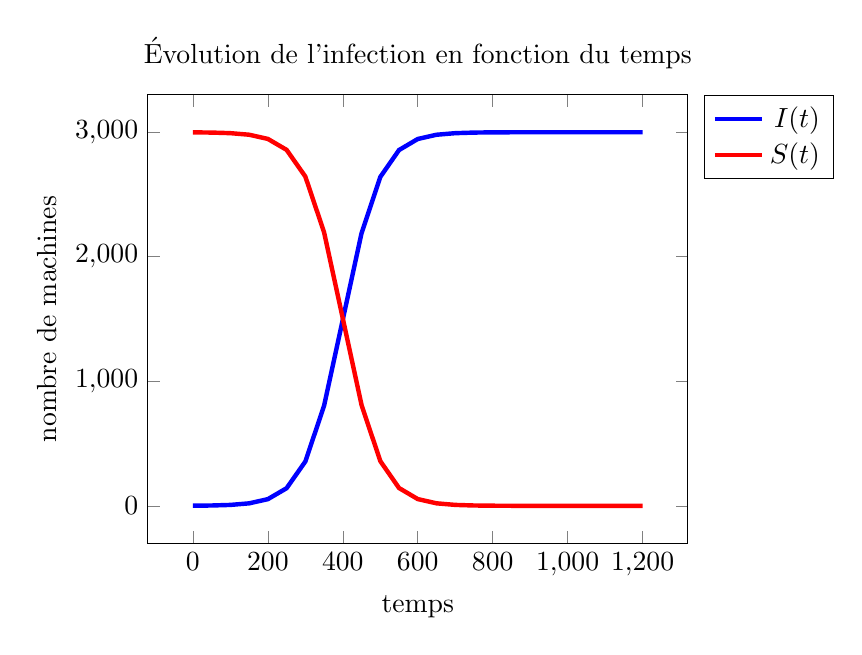
\begin{tikzpicture}[scale=1.0]
	\begin{axis}[
		title=Évolution de l'infection en fonction du temps,
		xlabel={temps},
		ylabel={nombre de machines},
		legend style={
			cells={anchor=east},
			legend pos=outer north east,},
		legend entries={$I(t)$,$S(t)$}
	]
		\addplot[domain=0:1200, blue, ultra thick] {3000/(2999*exp(-0.02*x)+1)};
		\addplot[domain=0:1200, red, ultra thick] {3000-(3000/(2999*exp(-0.02*x)+1))};
	\end{axis}
\end{tikzpicture}
}
\end{homeworkSection}

\begin{homeworkSection}{3.2}

Faites varier le paramètre  $\lambda (0.01, 0.025, 0.05)$. Représentez graphiquement les différentes courbes de $I(t)$ sur le même graphique. Commentez les différents graphiques obtenus en expliquant la signification quantitative du paramètre  et son impact sur la vitesse de propagation d'un vers. 

\end{homeworkSection}

\problemAnswer{
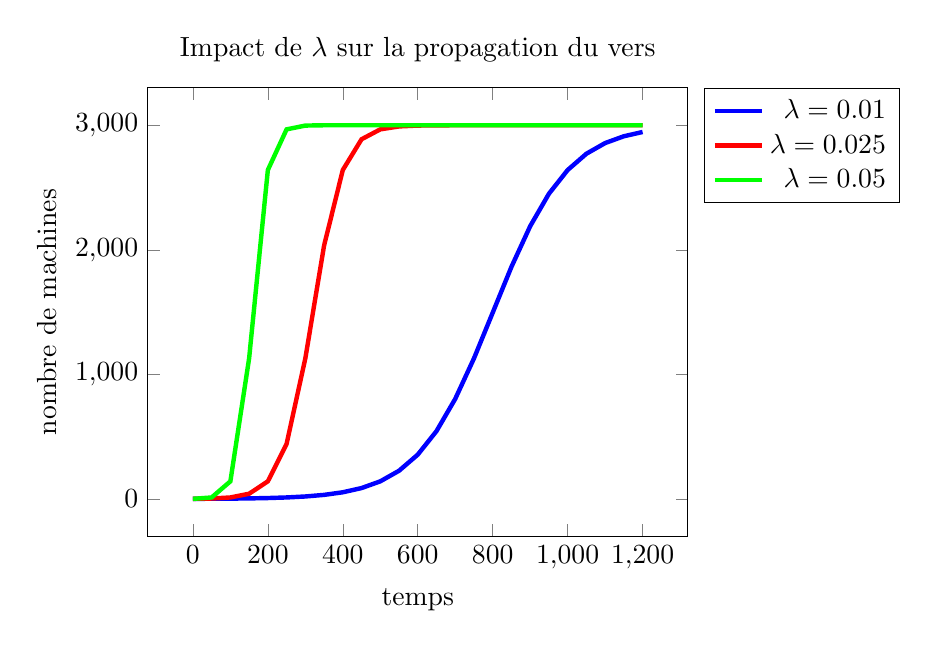
\begin{tikzpicture}[scale=1.0]
	\begin{axis}[
		title={Impact de $\lambda$ sur la propagation du vers},
		xlabel={temps},
		ylabel={nombre de machines},
		legend style={
			cells={anchor=east},
			legend pos=outer north east,},
		legend entries={$\lambda=0.01$,$\lambda=0.025$, $\lambda=0.05$}
	]
		\addplot[domain=0:1200, blue, ultra thick] {3000/(2999*exp(-0.01*x)+1)};
		\addplot[domain=0:1200, red, ultra thick] {3000/(2999*exp(-0.025*x)+1)};
		\addplot[domain=0:1200, green, ultra thick] {3000/(2999*exp(-0.05*x)+1)};
		
	\end{axis}
\end{tikzpicture}
\\

On remarque qu'avec un lambda plus élevé, la vitesse de propagation du vers est plus rapide.
$\lambda$ représente en fait le nombre d'interconnexion entre les sous réseaux.
Il est donc normal que plus qu'il est élevé, plus la propagation est rapide.
En effet, en partant d'un réseau à l'autre, si il y a moins d'interconnexion, il sera statistiquement plus long pour le vers de passer à l'autre sous réseau.
Ces graphiques montre donc que la réduction des interconnexions entre les réseaux est un bon moyen pour réduire la vitesse de propagation d'un vers. 
}
% %--------------------------------------------

% \begin{homeworkSection}{(a)} % Section within problem
% \lipsum[4]\vspace{10pt} % Question

% %\problemAnswer{ % Answer
% %\lipsum[5]
% %}
%\end{homeworkSection}

% %--------------------------------------------

% \begin{homeworkSection}{(b)} % Section within problem
% %\problemAnswer{ % Answer
% %\lipsum[6]
% %}
% \end{homeworkSection}

% %--------------------------------------------
\end{homeworkProblem}